\chapter{Linear Cross Entropy}
\label{ch:lxe}
\epigraph{Check the circuit}{Spock to helmsman;
  \citefield{butlerCage1988}{booktitle}
--- \citefield{butlerCage1988}{number}}

%In this chapter we examined the linear cross entropy in the projective
%transverse-field Ising model. The linear cross entropy was introduced by
%\citeauthor{liCrossEntropyBenchmark2023} in \cite{liCrossEntropyBenchmark2023},
%and first investigated for the projective transverse-field Ising model by
%\citeauthor{tikhanovskayaUniversalityCrossEntropy2023} in
%\cite{tikhanovskayaUniversalityCrossEntropy2023}. In search of a promising
%candidate for an order parameter of the phase transition that is measureable in
%an experimental setting, we picked up where these previous works left off. Our investigations
%PTIM: \cite{langEntanglementTransitionProjective2020}
%
%Fisher/Altman PRL, hier wird die LXE definiert: \cite{liCrossEntropyBenchmark2023}
%
%Nicolai: \enquote{Das ist eines der Paper, die Fisher zitiert, wo die LXE eingeführt wurde.} \cite{baoSymmetryEnrichedPhases2021}
%
%arXiv:2306.00058, LXE fürs PTIM, preprint \cite{tikhanovskayaUniversalityCrossEntropy2023}
%
%MIPT allgemein, hier leider eher weniger ahnung warum ich das in dieses Kapitel rein
%gemacht hab zum zitieren. \cite{baoTheoryPhaseTransition2020}
%
%Sampling stuff aus appendix von \cite{roserDecodingProjectiveTransverse2023}
%
%MOTHERFUCKER\ldots \cite{kamakariExperimentalDemonstrationScalable2024}

In this chapter we examine a measure known as the linear cross entropy proposed
by \citeauthor{liCrossEntropyBenchmark2023} in
\cite{liCrossEntropyBenchmark2023} to experimentally access measurement-induced
phase transitions. Despite its novelty, it has already been employed in
experiments to probe hybrid quantum circuits
\cite{kamakariExperimentalDemonstrationScalable2024}, and other theoretical
works are based on it. Even for our model system, the projective
transverse-field Ising model (PTIM), a study has been conducted (see Ref.
\cite{tikhanovskayaUniversalityCrossEntropy2023}\footnote{While this reference
  points to a preprint on arXiv, we remark that the cited work has since been
published in
\citefield{tikhanovskayaUniversalityCrossentropy$mathbbZ_2$2024}{journaltitle}
with no significant alterations (see Ref.
\cite{tikhanovskayaUniversalityCrossentropy$mathbbZ_2$2024}).}). With this in
mind we thus build on the work of
\citeauthor{tikhanovskayaUniversalityCrossEntropy2023} in
\cite{tikhanovskayaUniversalityCrossEntropy2023}. In particular, we reproduce
their findings, provide a more detailed insight into the features and
technicalities of the linear cross entropy, and further expand on their work by
introducing more general types of noise.
%reproducing their findings, and providing a more detailed insight into the
%technicalities of the linear cross entropy. 
We thereby aim to detect the theorized measurement-induced phase transition in
the projective transverse-field Ising model in the best case, or gain a new
understanding from failure in the worst case. 

%We particularily
%want to examine it for our model system, the projective transverse-field Ising
%model (PTIM), and evaluate its suitability to circumvent the sampling problem
%and detect the phase transition.
%for the projective transverse-field Ising model and evaluate its suitability to
%circumvent the sampling problem and detect the phase transition. This measure is called the \emph{linear
%cross entropy} (abbreviated as LXE). Although it is a novel quantity, its properties in hybrid
%circuits, and general random circuits, have already been explored in varying
%degrees of detail, with 
%Even for the projective transverse-field Ising model (PTIM),
%a study has been conducted . In the present
%chapter, we will investigate the properties of the linear cross entropy in
%general and for the projective transverse-field Ising model. We will also
%evaluate its quality as an order parameter for the phase transition of the
%PTIM.

The chapter is structured as follows. We will first introduce the quantity
itself in \cref{sec:lxe-defn}, where we also provide a shortcut for computing
the LXE in clifford circuits. We then investigate the behavior of it in the
PTIM, comparing it to the entanglement entropy of an ancilla qubit attached to
the system. Next, we introduce faulty gates to the process and examine the LXE
for a system with errors. Lastly, we motivate the discarding of either $X$ or
$ZZ$ measurement results with probability-theoretic arguments and evaluate the
utility of the LXE for the different cases.
\newpage
\section{Definition and properties}\label{sec:lxe-defn}
In this section we provide a definition for the linear cross entropy $\chi$
(also abbreviated as LXE)
and a detailed derivation for its computation in Clifford circuits. To this
end, we follow the results of Ref.
\cite{liCrossEntropyBenchmark2023,tikhanovskayaUniversalityCrossEntropy2023} for the
generalities, and provide our own derivations and proofs for the
particularities surrounding the projective transverse-field Ising model.

Before introducing all the technical details surrounding the linear cross
entropy, we want to give a quick remark on the motivation behind the linear
cross entropy. In Ref.
\cite{liCrossEntropyBenchmark2023}, they mention that eariler studies found a
quantity closely related to $-\ln\chi$ corresponding to the free energy cost
after fixing a boundary condition in a replicated spin model
\cite{liCrossEntropyBenchmark2023,baoTheoryPhaseTransition2020,jianMeasurementinducedCriticalityRandom2020,nahumOperatorSpreadingRandom2018,zhouEmergentStatisticalMechanics2019}.
The linear cross entropy is thus also motivated from classical statistical physics.
%Note that although the linear cross entropy was originally introduced in Ref. \cite{liCrossEntropyBenchmark2023}
%in a rather technical manner, they mention that earlier studies (see Ref.
%\cite{baoTheoryPhaseTransition2020}) have pointed out 
%that a quantity closely related to $-\ln\chi$ corresponds to the free energy
%cost of fixing a boundary condition in a 

\subsection{General random circuits}
We first introduce the linear cross entropy (also abbreviated as LXE) in the
context of general random quantum circuits. We then provide a concrete
description and expression of the LXE for our system, the projective
transverse-field Ising model.

Consider a hybrid circuit with some cicruit layout $C$, consisting of unitary
and measurement gates. The measurement gates within the circuit yield results
$m_i$, which are collected in the sequence $\mathbf{m} = \{m_1, m_2, \ldots,
m_N\}$, where $N$ is the number of measurement gates. We call this sequence of
measurement outcomes the \emph{measurement record}. For some initial state
$\rho$ of our hybrid circuit, we can compute the \emph{unnormalized} output
state as
\begin{align}\label{eq:rho-m}
  \rho_\mathbf{m} \equiv C_\mathbf{m} \rho C^\dagger_\mathbf{m}
.\end{align}
Here, $C_\mathbf{m}$ is the time-ordered product of all gates in the circuit,
unitary and measurement, and can be written as
\cite{liCrossEntropyBenchmark2023}
\begin{align}
  C_\mathbf{m} = \mathbb{P}_{m_N} \mathbb{P}_{m_{N-1}} \cdots
  \mathbb{P}_{m_{N-N_T+1}} U_T \mathbb{P}_{m_{N-N_T}} \cdots
  \mathbb{P}_{m_{N-N_T-N_{T-1}+1}} U_{T-1} \cdots
.\end{align}
The action of $C_\mathbf{m}$ on the initial state
$\rho$ is the mathematical object representing one possible trajectory with
measurement outcomes $\mathbf{m}$. Leaving the state unnormalized after 
projection operations is a deliberate choice; it allows us to define the
probability of a certian measurement record.

\begin{defn}[Probability of a trajectory]\label{defn:prob-traj}
  Given a random circuit $C$ and an initial state $\rho$ with corresponding
  measurement record $\mathbf{m}$, the probability of $\mathbf{m}$ is denoted
  by
  \begin{align}\label{eq:prob-traj-defn}
    P\left( \mathbf{m} \mid C, \rho \right) \equiv \Tr[\rho_\mathbf{m}] =
    \Tr[C_\mathbf{m} \rho C^\dagger_\mathbf{m}]
  .\end{align}
\end{defn}

Although we do not want to delve too deep into probability theory at this point,
let us nonetheless first convince ourselves that \cref{defn:prob-traj} really does
define a proper probability measure. To this end, consider the simplest example of
a circuit with initial state $\rho = \dyad{+}$ and a single measurement in the
Pauli-$Z$ basis. By \cref{eq:rho-m} our unnormalized output state reads
\begin{align}\label{eq:prob-example}
  \rho_\mathbf{m} = \mathbb{P}_m \dyad{+} \mathbb{P}_m^\dagger = \begin{cases}
    \frac{1}{2}\dyad{0}, & m = 1 \\
    \frac{1}{2}\dyad{1}, & m = -1
  \end{cases}
\end{align}
with $\mathbb{P}_m = \frac{1}{2}\left(\mathds{1} + m Z \right)$. Computing the
trace then yields $\frac{1}{2}$ for the probability of each trajectory. This is
also consistent with our expectation from elementary quantum mechanics. As
projectors sum to the identity (completeness), all the probabilities sum to
$1$, as they should.
Furthermore, since unitaries leave the norm invariant, the trace only picks up
projections. However, one needs to be careful here. Applying a Hadamard gate to
$\dyad{+}$ transforms the state, and the probabilities change.\footnote{The
  probabilities for the outcomes of a Pauli-$Z$ measurement become $1$ and
$0$}. Conversely,
applying a Hadamard gate to any of the output states in \cref{eq:prob-example}
does not alter the trace, but rather the output state itself.

We will later continue this discussion for the measurement-only circuit of the
PTIM. For now, we employ \cref{defn:prob-traj} and define the circuit-level
linear cross entropy $\chi_C\left(\rho, \sigma  \right)$.

\begin{defn}[Linear cross entropy]\label{defn:lxe}
  Given a random circuit $C$ with two distinct initial states $\rho$ and
  $\sigma$, and measurement records $\mathbf{m}$, the normalized linear cross
  entropy is defined as
  \begin{align}\label{eq:lxe-c-defn}
    \chi_C = \sum_{\mathbf{m}} P(\mathbf{m} \mid C, \rho) \frac{P(\mathbf{m} \mid
      C, \sigma)}{\sum_{\mathbf{m}'}\left(P(\mathbf{m}' \mid
      C, \sigma)\right)^2}
  ,\end{align}
  where the sums $\sum_\mathbf{m}$ go over all possible measurement outcomes of
  the measurement gates in the circuit.
\end{defn}
Most times when dealing with random circuits, we want to investigate numerous
different circuit realizations for a given parameter (usually probability).
Hence, when referring to the linear cross entropy, we will mostly refer to the
circuit-averaged linear cross entropy,
\begin{align}
  \chi \equiv \expval{\chi_C}_C
.\end{align}
We will later also see the utility of defining $\chi$ and $\chi_C$ this way,
especially concerning the denominator in \cref{eq:lxe-c-defn}. For now it
suffices to remark that it is a normalizing factor such that the linear cross
entropy is bounded from above by 1, $0 \leq \chi \leq 1$.

We can interpret this quantity like a classical fidelity between two
probability distributions. For two given initial states, we have a probability
distribution over measurement records. For each measurement record,
\cref{defn:prob-traj} provides a way to quantify the probability. For these
probabilities, the linear cross entropy quantifies the overlap of one
probability distribution with the other. If $\chi = 1$, the probability
distributions are identical, and if we chose different initial states, a unit
linear cross entropy tells us that this circuit (or parameter $p$) is not
suited to distinguish between the initial states $\rho$ and $\sigma$. On the
other hand, if $\chi=0$, we have no measurement record, which is compatible
with $\rho$ and $\sigma$ simultaneously.

\subsection{Clifford circuits and PTIM}\label{sec:lxe-for-ptim}
Now that we have introduced the general concept of the linear cross entropy and
defined the relevant quantities formally, we will examine it more closely in
the context of the projective transverse-field Ising model. As we are able to
simulate the PTIM with a stabilizer simulator, we will also introduce a way to
compute the LXE in Clifford circuits, which will be implemented in the
simulator.

In \cref{eq:lxe-c-defn}, the choice of placement of the individual
probabilities is a deliberate one. It is to highlight the fact that we are
averaging a quantity depending on $\sigma$ over a probability distribution that
depends on $\rho$. As a means of cirumventing the sampling problem, we'd like
$\sigma$ to correspond to a classical simulator and $\rho$ to the experiment.
It will therefore prove useful to examine the part dependent on $\sigma$ more
closely, as it will later enable us to efficiently compute the linear cross
entropy.
As intermediate step we first derive an
expression for the probabilities $P\left( \mathbf{m} \mid C, \rho \right)$,
laid out in \cref{lem:prob-traj-cliff}.
\begin{lem}[Probability of a trajectory in measurement-only Clifford circuits]\label{lem:prob-traj-cliff}
  Given a Clifford circuit $C$ with $N$ measurement gates and no other gates, with initial
  stabilizer state $\rho$, the probability of a measurement record is
  \begin{align}
    P\left(\mathbf{m} \mid C, \rho\right) = 2^{-N_\mathrm{rand}}
  ,\end{align}
  where $N_\mathrm{rand} \leq N$ is the number of random outcomes for the
  measurement gates.
\end{lem}

\begin{proof}
Suppose we have a Clifford circuit $C$ with $N$ measurement gates and an
$n$-qubit initial stabilizer state $\rho$. We already
know from \cref{sec:stabilizergroup} that there are two types of measurement
outcomes, random or deterministic. Each measurement potentially has 2 outcomes,
and in the former case each outcome has probability $1 / 2$ of occuring. (The
other outcomes, the deterministic ones, trivially have unit probability.)
Furthermore, we know that $\rho$ can be expressed as the product of projectors
(see \cref{defn:stab-dmat})
\begin{align}
  \rho = \frac{1}{2^n} \prod_{i=1}^n (I + g_i)
\end{align}
with generators $g_i$,
or equivalently as a sum of \emph{all} stabilizer group elements
\begin{align}
  \rho = \frac{1}{2^n} \sum_{g\in \mathcal{S}(\rho)} g
.\end{align}

If we now subject $\rho$ to the circuit $C$, we obtain a measurement record
$\mathbf{m}$. By \cref{defn:prob-traj} we compute the probability by tracing the
unnormalized output state (see \cref{eq:rho-m}), which in turn is obtained by application
of the respective projectors on the input state, i.e.
\begin{align}
  \rho_\mathbf{m} = C_\mathbf{m}\ \rho \ C_\mathbf{m}^\dagger 
  = T\left\{\prod_i^N\mathbb{P_i}\right\}\ \rho \ T\left\{\prod_i^N\mathbb{P_i}\right\}^\dagger 
.\end{align}
Here, $T\{\bullet\}$ is the time-ordering operator and $\mathbb{P}_i$ is the
projection operator on measurement outcome $i$. The probability of some
measurement record is then given by
\begin{align}
  P\left(\mathbf{m} \mid C, \rho\right) = \Tr[C_\mathbf{m} \rho
  C_\mathbf{m}^\dagger]
,\end{align}
which can be written as
\begin{align}
  P\left(\mathbf{m} \mid C, \rho\right) = \Tr[T\left\{\prod_i^N
  \mathbb{P}_i\right\}\rho]
,\end{align}
with the cyclic property of the trace and $\mathbb{P}^2 = \mathbb{P}$.
We can now consider the successive application of measurement gates.
We know that each of the $N$ measurements is either random or deterministic.
Let us therefore consider these two cases separately.
\par{Case 1 -- Deterministic outcome:}
If a measurement has a deterministic outcome, the measurement operator was
already part of the stabilizer group. We can therefore construct a set of
commuting operators $\langle g_i\rangle$, containing the measurement operator
$M$, which generate the
stabilizer group. If we let $g_1=M$ w.l.o.g., we have
\begin{align}
  P\left(\mathbf{m} \mid C, \rho\right) 
  &= \Tr[ \mathbb{P}_N \cdots \mathbb{P}_i \rho ] \nonumber\\
  &= \frac{1}{2^{n-1}}\Tr[\mathbb{P}_N \cdots \frac{1}{2} (I + M)\frac{1}{2} (I + g_1)
  \prod_{i=2}^n (I + g_i)] \nonumber\\
  &= \frac{1}{2^{n-1}}\Tr[\mathbb{P}_N\cdots \frac{1}{2}(I+M) \prod_{i=2}^n (I+g_i)] \nonumber\\
  &= \frac{1}{2^n}\TR[\mathbb{P}_N\cdots \mathbb{P}_{i+1} \prod_{i=1}^n
  (I+g_i)] \label{eq:prob-determ}
,\end{align}
where we used the fact that $\mathbb{P}^2 =\mathbb{P}$. The last line of
\cref{eq:prob-determ} tells us that deterministic measurements do nothing on
the state and the probability.
\par{Case 2 -- Random outcome:}
In the case of a random outcome, the operator to be measured was not in the
stabilizer group. Technically, it should be replaced, which is done by
conjugation with the projector. However, it turns out that for the probability,
we only need to consider a single projection. It is
\begin{align}
  P\left(\mathbf{m} \mid C, \rho\right) 
  &= \Tr[ \mathbb{P}_N \cdots \mathbb{P}_i \frac{1}{2^n}\sum_{g \in
  \mathcal{S}(\rho)} g]\nonumber\\
  &= \Tr[ \mathbb{P}_N \cdots \frac{1}{2} \left(\frac{1}{2^n} \sum_{g \in
  \mathcal{S}(\rho)} g + \sum_{g \in \mathrm{Stab}(\rho)} Mg\right) ]
.\end{align}
Since the second sum is exclusively one over Pauli matrices, which are traceless,
they don't contribute to the total. We thus have
\begin{align}
  P\left(\mathbf{m} \mid C, \rho\right) 
  = \Tr[\mathbb{P}_N \cdots \mathbb{P}_{i+1} \frac{1}{2^{n+1}}
  \sum_{g\in\mathcal{S}(\rho)} g]
.\end{align}

Combining cases 1 and 2, knowing that measurements with deterministic outcomes
don't alter the state at all, we have
\begin{align}
  P\left(\mathbf{m} \mid C, \rho\right) 
  &= \Tr[\frac{1}{2^{n+N_\mathrm{rand}}} \sum_{g\in\mathcal{S}(\rho)}
  g]\nonumber\\
  &= \frac{1}{2^{N_\mathrm{rand}}} = 2^{-N_\mathrm{rand}}
.\end{align}
%
%that each of the $N$ measurements is either a projection onto a stabilizer of
%$\rho$ or an alteration of the state in one or another way with probability $1
%/2$. Thus, any projection onto a measurement with deterministic outcome will
%act as identity on $\rho$. Consequently, we are left with $N_\mathrm{rand}$
%random outcomes to measurements, each of them with probability $1/2$. 
\end{proof}

We can now use this result to find a nice expression for the linear cross
entropy in Clifford circuits, and in particular the projective transverse-field
Ising model.
\begin{thm}[LXE for Clifford circuits]\label{thm:lxe-cliff}
  Let $C$ be a Clifford circuit with $N$ measurement gates and a measurement
  record $\mathbf{m}$ obtained from a realization of $C$ with some initial
  state $\rho$. Furthermore, let
  $\sigma \neq \rho$ be a different state, where $\mathbf{m}'$ are all possible
  measurement records from applying $C$ on $\sigma$. Then
  \begin{align}\label{eq:diesesding}
      \frac{P(\mathbf{m} |
      C,\sigma)}{\sum_{\mathbf{m'}}\left(P(\mathbf{m}'|C,\sigma)\right)^2}
      = \begin{cases}
        1 & \qquad{\sigma\text{ is compatible with }C \text{ and }
        \mathbf{m}}\\
        0 & \qquad{\sigma\text{ is not compatible with }C \text{ and }
        \mathbf{m}}\\
      \end{cases}
  .\end{align}
\end{thm}

\begin{proof}
  We can consider two (disjoint) cases:
  \begin{enumerate}
    \item No projection in $C_\mathbf{m}$ is orthogonal to $\sigma$, meaning
      that $\sigma$ is compatible with $C$ and $\mathbf{m}$.

      This implies that the trace in the computation of $P\left(\mathbf{m} \mid
      C,\sigma\right)$ will always be strictly above $0$. In fact, the
      probability will be $2^{N_\mathrm{rand}}$, since each projection was
      successful. Together with the fact that there are $2^{N_\mathrm{rand}}$
      measurement gates we have
      \begin{align}
      \frac{P(\mathbf{m} |
      C,\sigma)}{\sum_{\mathbf{m'}}\left(P(\mathbf{m}'|C,\sigma)\right)^2} =
      \frac{2^{-N_\mathrm{rand}}}{\sum_{\mathbf{m}'} 2^{-2N_\mathrm{rand}}}
      = \frac{2^{-N_\mathrm{rand}}}{2^{-N_\mathrm{rand}}} = 1
      .\end{align}

    \item At least one projection in $C_\mathbf{m}$ is orthogonal to $\sigma$,
      meaning that $\sigma$ is not compatible with $C$ and $\mathbf{m}$.

      Here we have at least one projection in $C_\mathbf{m}$, which projects
      $\sigma$ onto the $0$-vector. Incidentally, we require \emph{exactly} one
      projection to be orthogonal, since we then have no object that can be
      projected to anything. Thus, the trace becomes $0$, and as a consequence
      we have
      \begin{align}
      \frac{P(\mathbf{m} |
      C,\sigma)}{\sum_{\mathbf{m'}}\left(P(\mathbf{m}'|C,\sigma)\right)^2} = 0
      .\end{align}
  \end{enumerate}
\end{proof}

The second case in the proof of \cref{thm:lxe-cliff} is an interesting one to
consider, especially in the context of the PTIM. Suppose we run a PTIM circuit
on some $n$-qubit platform with an initial state of $\ket{\phi_0} = \left( \ket{0\cdots 0} +
\ket{1\cdots 1} \right) / \sqrt{2}$ or $\rho = \dyad{\phi_0}$. This produces a measurement record, which we
then feed into a classical simulator with an orthogonal Bell state
$\ket{\varphi_0} = \left( \ket{0\cdots 0} - \ket{1\cdots 1} \right) / \sqrt{2}$
or $\sigma = \dyad{\varphi_0}$.
There are of course other orthogonal Bell states we could choose as initial
state for our simulator. However, these two states are additionally orthogonal
in the logical basis. That is, if we encode information in $\ket{\phi_0}$, the
opposite information is encoded in $\ket{\varphi_0}$. That this choice is a
reasonable one gets even more apparent when considering generating sets of the
respective stabilizers,
\begin{align}\label{eq:rhosigmagenerators-lxe}
  \mathcal{S}_\rho = \langle X\ldots X, Z_1Z_2,\ldots,Z_{n-1}Z_n\rangle \quad{\text{and}}
  \quad
  \mathcal{S}_\sigma = \langle -X\ldots X, Z_1Z_2,\ldots,Z_{n-1}Z_n\rangle
.\end{align}
Notice that they are almost identical with a different sign in front of the
global $X$ stabilizer, implying orthogonality in the logical basis. In the
hypothetical, measurement outcomes of $\rho$ are projected onto $\sigma$.
Let us consider the two types of measurement, pairwise $ZZ$ and single-site
$X$. Performing a pairwise $ZZ$ measurement is a stabilizer measurement,
apparent from the generating sets given in \cref{eq:rhosigmagenerators-lxe}. A
measurement thereof will (at least initially) produce deterministic measurement
outcomes with $m = +1$. This is different for the $X$ measurements. Initially,
an $X$ measurement will not have an outcome we can infer beforehand. This,
however, is the case for both of them, up to a certain degree, since the
pairwise $Z$ stabilizers anticommute with the single-site $X$ measurement. This
also provides an explanation on why this is not always the case. If $X$
measurements are sufficiently frequent, there will be a point where there are
no $ZZ$ generators left, as all of them were replaced by $X$ by means of
measuring. Consequently, subsequent measurements of $X$ are deterministic,
which will detect the sign difference of the global $X$ stabilizer. This
detection would correspond to the point where the initial cluster dies in the
colored cluster model.

It turns out that this is the only case for the circuit-level linear cross
entropy to be $0$, i.e. $\chi_C = 0$. One can argue from the structure of the
stabilizer group, or just the generating set, that any measurements producing a
random outcome will produce a random outcome no matter what the previous
results were.\footnote{They are \enquote{Markovian} in that sense.} For an
outcome to be random, the measurement operator may not be contained in the
stabilizer of the state. Conversely, for an outcome to be deterministic, the
operator is a stabilizer. After measuring, the operator is guaranteed to be in
the stabilizer group of the state and subsequent measurements of this operator
produce the same result with unit probability. With the structure of the group
changed, we also have new anticommuting measurement operators, and so on. This
boils down to the conclusion that once the circuit $C$ is fixed, the
\emph{type} of measurement outcome is fixed. One could tell, without knowing
the actual outcomes to measurements, which of them were random and which were
deterministic. As such, a given circuit, which detects the sign difference
between $\sigma$ and $\rho$, does so in all of the runs, as deterministic
measurement outcomes stay so regardless of the previous history. Consequently,
the circuit-level linear cross entropy is $0$ regardless of measurement record
$\mathbf{m}$, if $C$ contains a deterministic measurement in $X$, where the
outcome is not given by a previous measurement, but by the sign of the initial
global $X$ stabilizer.

%We will henceforth refer to this mechanism of
%the linear cross entropy going to $0$ as mechanism \textsf{A}. As a
%visualization of this mechanism, confer with \cref{fig:mechanism-a}, showing a
%minimal example of a circuit detecting the sign difference.
\Cref{fig:mechanism-a} shows a minimal example of vanishing linear cross
entropy on the circuit level with initial states chosen as orthogonal Bell
states.

\begin{figure}[t]
  \centering
  \begin{tikzpicture}
  % Vertical separation between rho and sigma
  \draw[black,very thick] (5,0) -- (5,6.5);

  \node [init] at (2.5,.4) (rho) {$\rho$ (Experiment)\\$S = \langle
  +XX, ZZ\rangle$};
    %\\ $S_\rho = \langle X\ldots X,Z_1Z_2,
    %\ldots, Z_{n-1}Z_n\rangle$};
  \node [init] at (7.5,.4) (sigma) {$\sigma$ (Simulation)\\$S = \langle
  -XX,ZZ \rangle$};
    %\\ $S_\rho = \langle X\ldots X,Z_1Z_2,
    %\ldots, Z_{n-1}Z_n\rangle$};

  % rho
  \draw[black,thick] (2,1) -- (2,6);
  \draw[black,thick] (3,1) -- (3,6);

  \draw[gray, dashed] (.5,1.25) node[left] {$t=1$} -- (4.5,1.25) ; 
  \draw[gray, dashed] (.5,4.25) node[left] {$t=2$} -- (4.5,4.25); 

  %\filldraw [gray!128] (0.0, 3.25) circle [radius=1.2pt]
  %                     (0.4, 3.25) circle [radius=1.2pt]
  %                     (0.8, 3.25) circle [radius=1.2pt];
  %\filldraw [gray!128] (4.0, 3.25) circle [radius=1.2pt]
  %                     (4.4, 3.25) circle [radius=1.2pt]
  %                     (4.8, 3.25) circle [radius=1.2pt];

  % sigma
  \draw[black,thick] (7,1) -- (7,6);
  \draw[black,thick] (8,1) -- (8,6);

  \draw[gray, dashed] (5.5,1.25) -- (9.5,1.25); 
  \draw[gray, dashed] (5.5,4.25) -- (9.5,4.25); 

  % build circuit, rho
  \node [measx] at (2,2) (x1) {$+1$};
  \node [init] at (2.5,3.5) (rho1) {$S = \langle +X_1, +X_2 \rangle$}
  \node [measx] at (3,5.0) (x2) {$+1$};

  % build circuit, sigma
  \node [projxsucc] at (7,2) (x1-1) {$\mathbb{P}\left(+X\right)$};
  \node [init] at (7.5,3.5) (sigma1) {$S = \langle +X_1, -X_2 \rangle$}
  \node [projxfail] at (8,5.0) (x2-1) {$\mathbb{P}\left(+X\right)$};

\end{tikzpicture}

  \caption{Minimal example of a PTIM setup showcasing the mechanism behind
    vanishing LXE with
  $L=2$, $T=2$, and $p\neq 0$. The experimental circuit is shown on the left
  side.  In this particular circuit the initial Bell cluster dies in the first
  measurement layer by measuring $X$, and thus removing the singular $ZZ$
  stabilizers.  The $+1$ in the box refers to the actual outcome of the result.
  The circuit on the right corresponds to the post-processing algorithm with
  orthogonal initial state in the logical basis. Here we project onto the
  measurement results given by the measurement record, represented by
  $\mathbb{P}(+X)$. The second projection is unsuccessful, since we had a sign
  difference initially.}
  \label{fig:mechanism-a}
\end{figure}

\section{A first PTIM simulation}
%\textcolor{red}{hier ein LXE vs $S_E$ bildchen nicht vergessen, i guess?}

In this section we will examine the linear cross entropy in the context of our
model system, the projective transverse-field Ising model. In particular, we
will perform stabilizer simulations, as we have now
worked out how the LXE can be computed in the context of Clifford circuits. As we
also know an efficient method of computing the (experimentally inaccessible)
entanglement entropy, we will also compare the LXE with the entropy of
entanglement.
\subsection{Methods}\label{sec:lxe-numeric}
Before we discuss the linear cross entropy in detail, we introduce the setup
for our simulations. If not explicitly stated otherwise, the simulations were
performed with a stabilizer simulator written in \verb|C++| using the algorithm detailed in
\cref{ch:mixed,sec:tableau} \cite{langCliffordCircuitSimulator2022}.
Previous numerical investigations of the projective transverse-field Ising
model have that the sample average of a system is
\cite{roserDecodingProjectiveTransverse2023}
\begin{align}\label{eq:decoder}
      \expval{\expval{f_D}} = \sum_{\mathcal{T} \in \{
    \mathcal{T} \} } P\left(\mathcal{T}\right) \cdot
    f\left(\mathcal{T} ; D(S)\right)
,\end{align}
where $\mathcal{T}$ indicates a trajectory in the system and
$\{ \mathcal{T} \}$ is the set of all possible trajectories for a given
initial state. The double angled braces 
denote the average over both measurement records within one circuit as well as
circuits of a given probability. In the following we discuss how we should go
about sampling the circuits in order to get a sensible ensemble average, such
that we arrive at something of the form in \cref{eq:decoder}.

In \cref{eq:decoder}, a trajectory is defined as the circuit $C$, i.e. the measurement pattern,
and the outcomes of said measurements, $\mathbf{m}$, including the initial
state. A reasonable place to start is to find a probability we average over.
If we split the measurement record into disjoint records of $X$
measurements $\mathbb{m}_X$ and $ZZ$ measurements $\mathbb{m}_Z$, we have that
the probability of a trajectory is
\begin{align}
      P(\mathcal{T}) &=
      p^{\abs{\mathbf{m}_X}}(1-p)^{LT-\abs{\mathbf{m}_X}}\cdot
      p^{(L-1)T-\abs{\mathbf{m}_Z}}(1-p)^{\abs{\mathbf{m}_Z}}\cdot
      2^{-N_\mathrm{rand}} \nonumber\\ &= 
      p^{\abs{\mathbf{m}_X}+(L-1)T-\abs{\mathbf{m}_Z}}(1-p)^{LT-\abs{\mathbf{m}_X}+\abs{\mathbf{m}_Z}}\cdot2^{-N_\mathrm{rand}}
,\end{align}
where $L$ is the number of qubits (without periodic boundary conditions) and
$T$ the number of timesteps. This follows from the fact that we have
probability $p$ of $X$ measurements occuring and probability $1-(1-p) = p$ of
$ZZ$ no measurements occuring, with the converse for the exponent of $(1-p)$.
The factor $2^{-N_\mathrm{rand}}$ is from the fact that $N_\mathrm{rand}$ of
the occuring measurements are random in nature and thus contribute a
probability of $1 /2$ each.

However, recall that the quantity we really want to average (first over the
measurement records, then over circuits), is the quantity defined in
\cref{eq:diesesding}. From \cref{thm:lxe-cliff} we know that we can consider
each circuit exactly once, since for each circuit it will either give $0$ or
$1$. We should therefore think about how to average the quantity
\begin{align}
      f(\mathbf{m}, C_p, \sigma) = \frac{P(\mathbf{m} |
     C_p,\sigma)}{\sum_{\mathbf{m'}}\left(P(\mathbf{m}'|C_p,\sigma)\right)^2}
\end{align}
for a PTIM circuit $C_p$ with probability parameter $p$, giving the probability
of $X$ measurements being performed on each site. We thus have a system average
for the PTIM with initial state $\rho$ and probability parameter $p$,
\begin{align}
      \expval{\expval{f}}_{p,\rho} = \sum_{C_p} P(C_p) \sum_\mathbf{m}
      P(\mathbf{m} |C_p,\rho)\cdot f(\mathbf{m},C_p, \sigma)
.\end{align}

In principle, the sums over $C_p$ and $\mathbf{m}$, i.e. the sum over
$\mathcal{T}$, include \emph{all possible} circuits $C_p$ and
corresponding measurement outcomes $\mathbf{m}$. However, as already discussed,
this creates a lot of unnecessary redundancy; with stabilizer circuits, each
$\mathbf{m}$ contributes 
the same factor of
$2^{-\abs{N_\mathrm{rand}}}$ to the total probability, it doesn't change
anything to sample over it. Thus, we can instead opt for the generation of
random circuits and subjecting $\rho$ to them once. We then use a project
function (see \cref{alg:projection}) to verify if a different initial state
$\sigma$ is compatible with the measurement record obtained from applying $C$
on $\rho$.

In the stabilizer
formalism, projections can be done as efficiently as applying measurement
gates,
since the mechanism behind it is similar. However, we do not get a measurement
result, but rather obtain feedback on the success of the projection.
For a detailed introduction into the
simulation algorithm used in the numerical experiments, consult \cref{ch:mixed}
and in particular \cref{sec:purestates}, as well as \cref{alg:projection}.

The actual simulation of the PTIM with the computation of the linear cross
entropy is then done as follows. First, as outlined in \cref{sec:the-ptim},
we generate two binary matrices of size $T\times L$, representing the
locations of $X$ and $ZZ$ measurements, respectively. We also initialize two
additional matrices of the same size to 0, where the measurement outcomes of
the respective run is stored. We then simulate a PTIM with a stabilizer
simulator (see Ref. \cite{langCliffordCircuitSimulator2022} and
\cref{ch:mixed}). Afterwards we repeat the
circuit for the other initial state, but use the measurement results in the
\enquote{outcome matrices} as argument for the project function. If at any
point during the simulation we encounter a failed projection, the loop over the
circuit stops and continue with the next one. If it successfully completes, we
add $1$ to the total and repeat the procedure for the next circuit.

Consequently, we technically compute the quantity
\begin{align}\label{eq:sample-f-C}
  \expval{\expval{f}}_{p,\rho} = \sum_{C_p} P(C_p) \cdot f(\mathbf{m},C_p,
  \sigma)
,\end{align}
when sampling for the linear cross entropy numerically, where we generate $C_p$
as a random circuit in our simulator. 

In the following, we will drop the index $p$ from the labelling of the circuit
$C_p$ for the sake of readability. It is nonetheless implied, and should be
clear from context that $C$ is a circuit randomly generated from a probability
parameter $p$.

\subsection{Results}

%\textcolor{red}{vielleicht hier nicht der erste hinweis darauf, dass da schon
%  peer-reviewed stuff in der welt rumgeistert, auf dem die ganze analyse
%basiert}
As \cite{tikhanovskayaUniversalityCrossEntropy2023} already explored
the linear cross entropy on the projective transverse-field Ising model, we
choose the identical setup with the maximally entangled states $\rho = \dyad{GHZ+}$ and
$\sigma = \dyad{GHZ-}$ as initial states with $L=T$ for better comparability
with their results in this and the upcoming sections of this chapter.

\Cref{fig:lxe-vs-se-default} shows the linear cross entropy and the
entanglement entropy for different system sizes.
\begin{figure}[h]
  \centering
  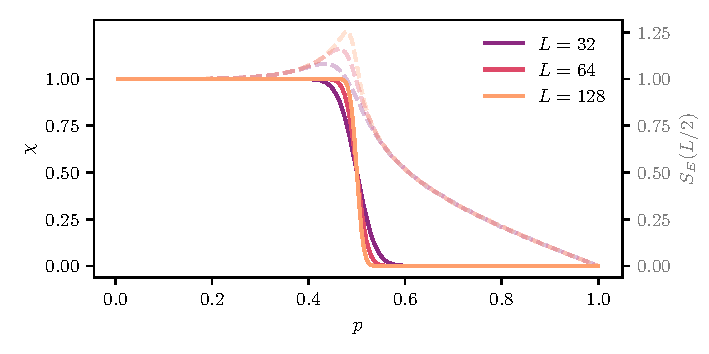
\includegraphics{no_error-track_all-lxe_vs_se.pdf}
  \caption{Linear cross entropy and entanglement entropy in the projective
  transverse-field Ising model and for $L=T$ and initial states $\rho =
  \dyad{GHZ+}$ for the actual system and $\sigma=\dyad{GHZ-}$ for the classical
  replica. Note that we here use open boundary conditions. For each probability
  parameter $p$, we sampled over $\sim 10^5$ circuit realizations.}
  \label{fig:lxe-vs-se-default}
\end{figure}

From \cref{fig:lxe-vs-se-default} one can see that the linear cross entropy
acts as an order parameter for the phase transition, with every line coinciding
at the critical point. One can also see that the linear cross entropy converges
faster towards the critical point than the entanglement entropy. The
entanglement entropy is still somewhat smooth at the critical point, while the
linear cross entropy is already smoothed out. This is due to the fact that the
LXE probes the survival of an initial entanglement cluster, while the
entanglement entropy quantifies independent entanglement pairs at the very end
of the circuit. As such, the linear cross entropy in this form is equivalent to
the entanglement entropy of an ancilla qubit entangled initially to the rest of
the system. We will make use of this fact later to test the reliability of the
LXE in the presence of noise.

A more subtle fact we do not want to fail to mention is that the entanglement
entropy is off-center in the case of open boundary conditions. In case of
periodic boundary conditions, we have the transition in the entanglement
entropy centered at the critical point.
We highlight both the convergence behavior and the shift of the critical point
in \cref{fig:lxe-closer-at-crit}. Note that we also use larger system sizes
compared to \cref{fig:lxe-vs-se-default}.

\begin{figure}[h]
  \centering
  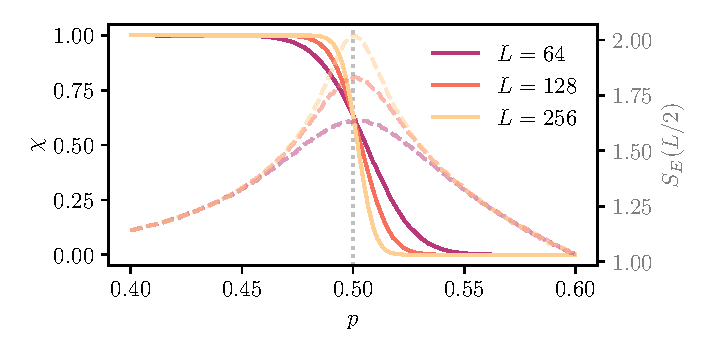
\includegraphics{lxe_closer_at_crit_pbc.pdf}
  \caption{Linear cross entropy and entanglement entropy zoomed in at the
  critical point for periodic boundary conditions. The dotted vertical line
corresponds to the theoretical critical point of the PTIM in the steady state.
Each datapoint corresponds to $\sim 10^5$ circuit realizations per probability
parameter.}
  \label{fig:lxe-closer-at-crit}
\end{figure}

What \cref{fig:lxe-closer-at-crit} also remarkably shows is that with periodic
boundary conditions $\chi(p=1 /2) > 1 /2$, whereas with open boundary
conditions it was $\chi(p=1 /2) = 1 /2$. The latter implies that half of the
initial clusters do not survive at the critical point, while the other half
does. With periodic boundary conditions, we add another source for stabilizer
measurements, thus leading to a more stable cluster towards the critical point,
which is still $p_c = 1 /2$. 
%\begin{itemize}
%  \item LXE converges faster than entanglement entropy, since the logarithmic
%    divergence at the critical point is not yet reached, but is rather smoothed
%    out
%  \item PBC vs OBC alter the behavior of the LXE slightly, as can be seen by a
%    more closer inspection in the regime, where one expects the critical point
%
%  \item Plot the above point (plot exists almost)
%    
%  \item Interpretation of fisher and the likes
%    \cite{liCrossEntropyBenchmark2023}: $-\log \chi$ is something like
%    a free energy difference, which would make the LXE something like a
%    partition function, since $F = \expval{E} - \beta^{-1}S = -\beta^{-1}\ln
%    Z$.
%
%  \item exponential scaling at critical point, also from fisher
%\end{itemize}

\section{Marinalizing over probabilities}\label{sec:lxe-indep}
In \cite{tikhanovskayaUniversalityCrossEntropy2023} they argue that
by tracking only the outcomes of $X$ measurements, one obtains the identical
results for the linear cross entropy compared to tracking all results.
In this section, we will
prove this statement with arguments from classical probability theory,
using that the probability $P(\mathbf{m} \mid C, \bullet)$ is a joint probability
distribution of two discrete random variables $\mathbf{m}_X$ and
$\mathbf{m}_Z$. 

The group theoretic arguments leading to vanishing linear cross entropy also
give rise to another insight into a more subtle property thereof. Since the
sign difference in the initial states is in the global $X$ stabilizer, we can
be certain of the fact that it must be an $X$ measurement, which failed to
project, thus leading to a vanishing linear cross entropy. Furthermore, we
argued that the type of a measurement (random or deterministic) is not altered
by previous measurements. (Note that this fact is completely independent of the
initial state!)
It will therefore prove useful to write the entire
measurement record as $\mathbf{m} = \mathbf{m}_X \cap \mathbf{m}_Z$, where
$\mathbf{m}_{X/Z}$ are the measurement records of $X$ and $ZZ$. The individual
outcomes in $\mathbf{m}$ are independent of their preceeding outcomes. It
follows that $\mathbf{m}_X$ and $\mathbf{m}_Z$ are independent random variables. 
Starting with orthogonal $GHZ$ states, we
could then, theoretically, marginalize over $\mathbf{m}_Z$ and should arrive at
the same linear cross entropy.

Let us consider what it implies to have independent random
variables.
Probability theory tells us that for independent random variables $A$ and $B$
we have $P(A, B) = P(A)P(B)$, which gives us
\begin{align}
      P(\mathbf{m} | C, \rho) = P(\mathbf{m}_X \cap \mathbf{m}_Z | C, \rho) =
    P(\mathbf{m}_X | C, \rho)\cdot P(\mathbf{m}_Z | C, \rho)
.\end{align}

Note that this argument relies on the fact that in \cref{eq:prob-traj-defn} we replace each measurement we
want to marginalize by an identity of the form
\begin{align}
  \mathds{1} = \mathbb{P}_+ + \mathbb{P}_-
,\end{align}
with the projectors onto measurement results $m_{X /Z} = \pm 1$. The sum that
emerges when all $X$ ($ZZ$) projections are replaced by this identity is then
the marginalized probability distribution of $ZZ$ ($X$).

Since the linear cross entropy solely consists of probabilities of this form,
we can insert above separation into \cref{eq:lxe-c-defn} to yield
\begin{align}
      \label{eq:lxe-subset}
      \chi_C &= \sum_{\mathbf{m}} P(\mathbf{m} \mid C, \rho) \frac{P(\mathbf{m} \mid
      C, \sigma)}{\sum_{\mathbf{m}'}\left(P(\mathbf{m}' \mid
      C, \sigma)\right)^2} \nonumber\\
      \nonumber\\
      &= \sum_{\mathbf{m}_X \cap \mathbf{m}_Z} P(\mathbf{m}_X \cap \mathbf{m}_Z |
        C, \rho) \frac{P(\mathbf{m}_X \cap \mathbf{m}_Z| C,
        \sigma)}{\sum_{\mathbf{m}_X' \cap \mathbf{m}_Z'} \left(P(\mathbf{m}_X' \cap
        \mathbf{m}_Z'|C,\sigma)\right)^2}\nonumber\\
        \nonumber\\
      &= \sum_{\mathbf{m}_X \cap \mathbf{m}_Z} P(\mathbf{m}_X | C, \rho) P(
        \mathbf{m}_Z | C, \rho) \frac{P(\mathbf{m}_X | C, \sigma) P( \mathbf{m}_Z|
        C, \sigma)}{\sum_{\mathbf{m}_X' \cap \mathbf{m}_Z'}
          \left(P(\mathbf{m}_X' | C,
        \sigma) P( \mathbf{m}_Z'|C,\sigma)\right)^2}\nonumber\\
        \nonumber\\
      &= \underbrace{\frac{\sum_{\mathbf{m}_Z} P(\mathbf{m}_Z | C, \rho)
          P(\mathbf{m}_Z | C, \sigma)}{\sum_{\mathbf{m}_Z'}
          \left(P(\mathbf{m}_Z' |
          C, \sigma)\right)^2}}_{\text{Subset ZZ}}
          \underbrace{\frac{\sum_{\mathbf{m}_X} P(\mathbf{m}_X | C, \rho)
          P(\mathbf{m}_X | C, \sigma)}{\sum_{\mathbf{m}_X'}
          \left(P(\mathbf{m}_X' |
          C, \sigma)\right)^2}}_{\text{Subset X}}
\end{align}
with \enquote{Subset ZZ} and \enquote{Subset X} being the marginalized versions
of the linear cross entropy, where the other type of measurement is traced out.

As of yet, we have not proven the statement that tracking the outcomes of $X$
measurements yields the same linear cross entropy as tracking all outcomes of
all measurements. We have only shown that when tracking only a subset of
measurements, we can multiply it by the complement to obtain the full linear
cross entropy.

However, if we paradigmatically start the circuit in orthogonal GHZ states,
where the only difference between the two initial states (the one of the
quantum and the one of the classical simulator) is the sign of the global $X$
stabilizer, we can deduce that there will never be a difference in the
\enquote{Subset ZZ} linear cross entropy, since replacing the projectors onto
$X$ measurement results by an identity will never project onto $0$. Therefore,
it should be identically $1$.

%It would therefore not make a difference if we
%would replace all projections onto $ZZ$ results to an identity. This argument
%boils down to a marginalization over $ZZ$ results, 
%This argument
%can be shown mathematically by considering the 
%\begin{align}
%  P\left( \mathbf{m} \mid C, \sigma \right) = \Tr[\mathbb{P}_N \cdots
%  \frac{1}{2} \left( \mathds{1} + ZZ \right) ]
%.\end{align}
%Thus, it would not make a difference if the
%results of $ZZ$ measurements in the circuit are projected onto $\sigma$ or if
%we 

\subsection{Methods and results}

To implement a marginalized version of the linear cross entropy, we need to
replace each projection we would perform in the replicated circuit by an
identity operation. Naively, we could then just remove all complementary
measurement gates in the numerical implementation. For a more accurate
description, or simulation, of what we actually want to achieve, we replace
each projection we would do when tracking all outcomes with a measurement gate,
where we choose to be agnostic to the outcome. This is done to keep the
underlying group structure intact. Note that contrary to the projection
operation we implemented, a measurement can always be performed and always has
an outcome.

For the results of a simulation implemented this way, consider the first row of subplots in
\cref{fig:err-vs-tra}. In this figure, we show the linear cross entropy as a
function of the probability parameter $p$, where the different columns
correspond to different marginalizations. We additionally plot the entanglement
entropy of an ancilla qubit entangled to the initial Bell cluster of the
system, as we already noted that this is a physically equivalent quantity in
this case.
In column \enquote{Track $X$ ($ZZ$)}
we only store the measurement outcomes of $X$ ($ZZ$) measurements and perform a
measurement of $ZZ$ ($X$) instead of a projection in the \enquote{classical
version} of the circuit. 

Note that the label \textsf{A} in the subplot of
columns $X$ and all correspond to the mechanism, which leads to a vanishing
cross entropy we discussed earlier and which is depicted schematically in
\cref{fig:mechanism-a}. The reason we introduce this becomes apparent in the
next section, where we examine the behavior of the linear cross entropy in the
presence of symmetric (projective) noise. For the noiseless case, the
previously introduced mechanism, which we will refer to as mechanism
\textsf{A}, is the only way where the linear cross entropy vanishes.

The first row in \cref{fig:err-vs-tra} clearly shows that only tracking the outcomes
of $ZZ$ measurements yields a (marginalized) linear cross entropy that is
identically 1. Conversely, the tracking of only the outcomes of $X$
measurements yields the same curve as the one where we track everything. This
is an indicator that the probability theoretic argument that $\mathbf{m}_X$ and
$\mathbf{m}_Z$ are independent random variables holds water. By our choice of
initial states, there is no mechanism present in the circuit, where the
marginalized cross entropy of $ZZ$ goes to 0. We will take special note of this
fact when we introduce noise to the circuit.
%\Cref{fig:lxe-no-error-tracks} shows the LXE for different marginalized
%probability distributions.
%\begin{figure}[h]
%  \centering
%  
\includegraphics[width=0.8\textwidth]{Untitled.png}
%  \caption{Hier erste zeile vom grossen tableau, damit klar ist, dass track
%  $ZZ$ identisch 1 ist und das dann beim actual tableau auff\"allt}
%  \label{fig:lxe-no-error-tracks}
%\end{figure}

\section{PTIM with faulty gates}
So far, the LXE appears to be a promising candidate for the order parameter of
the phase transition in the projective transverse-field Ising model.
Nevertheless, it is a well known fact that the world is not perfect. It is
utopian to imagine a quantum simulator going through a circuit without any
errors. Hence it seems a worthwile endeavor to investigate the robustness of the
linear cross entropy when the \enquote{experimentally realized} circuit with initial state $\rho$ is
subjected to noise.

In this section and the remainder of this chapter we investigate the
impact of a type of error model on the linear cross entropy and verify its
robustness to noise. We build on and critique the work of Ref.
\cite{tikhanovskayaUniversalityCrossEntropy2023} insofar as we
implement their error model in our simulations, expand it to include also $ZZ$
noise, as well as the marginalized linear cross entropies, and contextualize
the results.
\clearpage
\subsection{Error model}\label{sec:errormodel}

As error model, we implement the model from
\cite{tikhanovskayaUniversalityCrossEntropy2023}, where they
considered symmetric noise in $X$. The protocol to introduce errors is as
follows. Between each timestep, apply a quantum channel of the form
\begin{align}\label{eq:noisechannel}
  \varepsilon(\rho) = \frac{1}{2}\rho + \frac{1}{2}X\rho X
\end{align}
on each qubit with an error rate $q$.\footnote{We refer to this quantum channel
as \enquote{error} and \enquote{noise} interchangeably.} That is, after each timestep, before
applying the measurement gates of the next one, we construct an additional
measurement layer, where measurements of certain types are performed with
probability $q$.  This scheme is generic insofar as we can also imagine $ZZ$
errors happening in this way, as well as errors on both observables.

This type of error can be interpreted as additional measurements we failed to
keep track of in general, and not by choice. Another way of interpreting it is
that they constitute projective errors, akin to the one shown in a minimal
example in \cref{fig:error-detection-circuit}. Our expectation from the
interpretation of the survival rate of the initial cluster would be that for
$X$ noise, we have the phase transition at a smaller probability, since the
initial cluster dies earlier due to the presence of more frequent $X$
measurements. In the converse we expect the cluster to survive longer, since we
artificially introduce stabilizer measurements at a rate $q$.

Before we put this expectation to the test, we need to consider how we go about
sampling this quantity. We implement this noise in a way closest to what one
could consider noise in a real experiment starting with our usual scheme of
designing a random circuit $C$ and measuring accordingly. However, this time we
measure additionally on each qubit after each timestep with an error rate $q$.
These measurements we don't keep track of and seed randomly in the simulation
of $\rho$.

By introducing errors to the circuit, we subject it to quite impactful
alterations. Previously we could consider the reduced measurement
pattern---which we had access to---and apply it to both initial states, with
mechanism \textsf{A} being the only source of vanishing terms in the sampling.
Now we need to consider the designed, albeit still randomly generated, circuit $C$
and the faulty pattern $\tilde{C}$, where $\tilde{C}$ is parametrized by both
$p$ and $q$. Crucially, the new faulty circuit $\tilde{C}$ constitutes a
superset of $C$, since each measurement of $C$ is performed regardless. That
is, we have $C\subseteq\tilde{C}$. 

Note that this leaves the fraction in \cref{eq:lxe-c-defn,eq:diesesding}, that
is,
\begin{align}
      f(\mathbf{m}, C, \sigma) = \frac{P(\mathbf{m} |
     C,\sigma)}{\sum_{\mathbf{m'}}\left(P(\mathbf{m}'|C,\sigma)\right)^2}
\end{align}
invariant;
we are still trying to find the compatibility
between classical simulation $(C, \sigma)$ and \enquote{quantum} experiment
$(\tilde{C}, \rho)$.  However, we will obtain a different expression for the
sample average, \cref{eq:sample-f-C}. As we are trying to realistically
model errors, we should be unaware of the location they happen in, but assume
that they happened. As such, $\tilde{C}$ is a random circuit with probability
parameters $p$ and $q$ for measurements we do and do not have control over, respectively.
\Cref{eq:sample-f-C} then becomes a sum over $\tilde{C}_{p,q}$,
\begin{align}
  \label{eq:sample-f-Ctilde} \expval{\expval{f}}_{p,q,\rho} =
\sum_{\tilde{C}_{p,q}} P(\tilde{C}_{p,q}) \cdot f(\mathbf{m},C_p, \sigma)
.\end{align}

With the sampling scheme defined in a more precise way, we can refine our
predictions on the results in the simulation. Although the $f$ in
\cref{eq:sample-f-Ctilde} and \cref{eq:sample-f-C} are identical, the
measurement record we take as input is not generated from the same circuit.
Consequently, we can now identify other causes of the function going to $0$.

Previously we argued that the probability of a
measurement outcome is not influenced by preceeding measurements, that is, they
are independent random variables. While this is still the case, the argument
only holds on a circuit-level. The only way where an error does not alter the
probability of the succeeding measurements is, if it commutes with the
measurement operators on the same site that directly preceed or succeed the
error. For instance, if the circuit dictates a measurement of $X$, which is
then followed by the noise channel, the state is not altered and nothing is
affected.

Thus, we argue that there is an additional mechanism for vanishing
circuit-level linear cross entropy, where an error is not bypassed by the
mechanism described above, but is entrapped by the competing measurement.

Take, for instance, the minimal example of two qubits with $X$-Errors.
A valid measurement pattern would be $(Z_1Z_2, Z_1Z_2)$. Starting with a
Bell state would yield the outcomes $(+1, +1)$ deterministically. If
we now squeeze an error inbetween the two measurements, we have halved the
probability of getting $+1$ at the second timestep. Thus, for half of the runs
we would get an unsuccessful projection. 

\begin{figure}[t]
  \centering
  \begin{tikzpicture}
  % Vertical separation between rho and sigma
  \draw[black,very thick] (5,0) -- (5,6.5);

  \node [init] at (2.5,.5) (rho) {$\rho$ (Experiment)};
    %\\ $S_\rho = \langle X\ldots X,Z_1Z_2,
    %\ldots, Z_{n-1}Z_n\rangle$};
  \node [init] at (7.5,.5) (sigma) {$\sigma$ (Simulation)};
    %\\ $S_\rho = \langle X\ldots X,Z_1Z_2,
    %\ldots, Z_{n-1}Z_n\rangle$};

  % rho
  \draw[black,thick] (2,1) -- (2,6);
  \draw[black,thick] (3,1) -- (3,6);

  \draw[gray, dashed] (.5,1.25) -- (4.5,1.25); 
  \draw[gray, dashed] (.5,4.25) -- (4.5,4.25); 

  %\filldraw [gray!128] (0.0, 3.25) circle [radius=1.2pt]
  %                     (0.4, 3.25) circle [radius=1.2pt]
  %                     (0.8, 3.25) circle [radius=1.2pt];
  %\filldraw [gray!128] (4.0, 3.25) circle [radius=1.2pt]
  %                     (4.4, 3.25) circle [radius=1.2pt]
  %                     (4.8, 3.25) circle [radius=1.2pt];

  % sigma
  \draw[black,thick] (7,1) -- (7,6);
  \draw[black,thick] (8,1) -- (8,6);

  \draw[gray, dashed] (5.5,1.25) -- (9.5,1.25); 
  \draw[gray, dashed] (5.5,4.25) -- (9.5,4.25); 

  % build circuit, rho
  \node [measzz] at (2.5,2) (zz1) {$\mathcal{M}_{ZZ}=+1$};
  \node [errx] at (2,3.75) (xerr) {$X$};
  \node [measzz] at (2.5,5.0) (zz2) {$\mathcal{M}_{ZZ}=-1$};

  % build circuit, sigma
  \node [projzzsucc] at (7.5,2) (zz1-1) {$\mathbb{P}\left(+ZZ\right)$};
  \node [projzzfail] at (7.5,5.0) (zz2-1) {$\mathbb{P}\left(-ZZ\right)$};

\end{tikzpicture}

  \caption{Excerpt of a possible PTIM circuit with non-zero probability of
  $X$-errors occuring showcasing mechanism \textsf{B1}. At timestep $t=i$, 
  we perform a $ZZ$ measurement on two neighboring qubits with result $+1$,
  and an $X$-error occurs on the first qubit after the measurement. Then in the next
  timestep, we measure $ZZ$ once more. As a consequence of the error, this $ZZ$
  measurement is not deterministically $+1$, but randomly $\pm 1$ with
  probability $\frac{1}{2}$. When trying to project in the classical
  simulation, this discrepancy gets noticed, since we do not have access to the
  precise nature of the errors. Upon failed projection we have $\chi=0$.}
  \label{fig:mech-b1-lxe}
\end{figure}

\begin{figure}[t]
  \centering
  \begin{tikzpicture}
  % Vertical separation between rho and sigma
  \draw[black,very thick] (5,0) -- (5,6.5);

  \node [init] at (2.5,.4) (rho) {$\rho$ (Experiment)\\$S = \langle
  +XX, ZZ\rangle$};
    %\\ $S_\rho = \langle X\ldots X,Z_1Z_2,
    %\ldots, Z_{n-1}Z_n\rangle$};
  \node [init] at (7.5,.4) (sigma) {$\sigma$ (Simulation)\\$S = \langle
  -XX,ZZ \rangle$};
    %\\ $S_\rho = \langle X\ldots X,Z_1Z_2,
    %\ldots, Z_{n-1}Z_n\rangle$};

  % rho
  \draw[black,thick] (2,1) -- (2,6);
  \draw[black,thick] (3,1) -- (3,6);

  \draw[gray, dashed] (.5,1.25) node[left] {$t=i$} -- (4.5,1.25) ; 
  \draw[gray, dashed] (.5,4.25) node[left] {$t=i+1$} -- (4.5,4.25); 

  %\filldraw [gray!128] (0.0, 3.25) circle [radius=1.2pt]
  %                     (0.4, 3.25) circle [radius=1.2pt]
  %                     (0.8, 3.25) circle [radius=1.2pt];
  %\filldraw [gray!128] (4.0, 3.25) circle [radius=1.2pt]
  %                     (4.4, 3.25) circle [radius=1.2pt]
  %                     (4.8, 3.25) circle [radius=1.2pt];

  % sigma
  \draw[black,thick] (7,1) -- (7,6);
  \draw[black,thick] (8,1) -- (8,6);

  \draw[gray, dashed] (5.5,1.25) -- (9.5,1.25); 
  \draw[gray, dashed] (5.5,4.25) -- (9.5,4.25); 

  % build circuit, rho
  \node [measx] at (2,2) (x1) {$+1$};
  \node [errzz] at (2.5,3.5) (zzerr) {$ZZ$};
  \node [measx] at (2,5.0) (x2) {$-1$};

  % build circuit, sigma
  \node [projxsucc] at (7,2) (x1-1) {$\mathbb{P}\left(+X\right)$};
  \node [projxfail] at (7,5.0) (x2-1) {$\mathbb{P}\left(-X\right)$};

\end{tikzpicture}

  \caption{Excerpt of a possible PTIM circuit with non-zero probability of
    $ZZ$-errors occuring showcasing mechanism \textsf{B2}. At timestep $t=i$,
    we perform an $X$ measurement on the left qubit with result $+1$, and a
    $ZZ$ error occurs on the shown pair after the measurement. Then in the next
    timestep, we measure $X$ on the left qubit once more. As a consequence of
    the error, this $X$ measurement does not yield $+1$ deterministically, but
    $\pm 1$ with probability $\frac{1}{2}$ for either result. When trying to
    project in the classical simulation, this discrepancy gets noticed, since we
    do not have access to the precise nature of the errors. Upon failed projection
    we have $\chi=0$.}
  \label{fig:mech-b2-lxe}
\end{figure}

The mechanism of the circuit-level linear cross entropy going to $0$ due to
errors which fail to not get noticed will henceforth be denoted with
\textsf{B1} and \textsf{B2} for $X$-errors and $ZZ$-errors respectively.
Possible examples of them occuring in a PTIM experiment with the corresponding simulation
are depicted schematically in \cref{fig:mech-b1-lxe,fig:mech-b2-lxe}.

It is not hard to convince oneself that the linear cross entropy sampled with
faulty circuits is less than or equal to the original cross entropy, since the
original source of it going to $0$ is still present nonetheless. We can do a
simple estimation on the probability of one of the above introduced mechanisms
to bound the error-influenced linear cross entropy from above. These
considerations also serve to better understand them.

Let us consider mechanism \textsf{B1}, where $X$ errors occur with probability
$q$.
The measurement record $\mathbf{m}$ obtained from $\tilde{C}$ applied on $\rho$
is incompatible with $\sigma$ if there is a projection onto the zero-vector.
Thus, for a non-zero LXE we want this \emph{not} to happen. One way for this to happen
is if mechanism \textsf{B1} takes effect. To derive the probability of
\textsf{B1} occuring, consider the following train of thought.

\begin{enumerate}
  \item Two successive $ZZ$ measurements must occur in $C$ on the same edge. This event has probability
    $(1-p)\cdot (1-p)= (1-p)^2$ by the construction rules of the PTIM circuit.
  \item No $X$ measurements on the site where the error occurs. This event also
    has probability $(1-p)^2$, as $p$ is the probability of $X$ measurements,
    again by the rules on how we construct a PTIM circuit.
  \item An error must occur on one of the sites, which gets detected. The error
    rate is $q$, with an effective probability of $q /2$, since the
    \enquote{correct} measurement result is still a valid outcome in the
    circuit.
  \item The mechanism is symmetric in the two sites encompassed in the edge the
    $ZZ$ measurements occur, which multiplies the above points by 2.
\end{enumerate}

Thus, the probability of \textsf{B1} is
\begin{align}
  P(\textsf{B1}; p,q) = \frac{2}{2} q \left(1-p\right)^2\left(1-p\right)^2 = q\left(
  1-p\right)^4
.\end{align}
Since this should not happen anywhere in the space-time lattice, we have
\begin{align}\label{eq:lxe-estimate}
      \chi \leq \left( 1-q\left( 1-p \right)^4  \right)^{(L-1)(T-1)}
\end{align}
as an estimation for the linear cross entropy for $X$-errors.
The LXE is thus exponentially suppressed for $p<1$ in the thermodynamic limit
of $L \to \infty$. We should also not confuse the facts here; this estimate
does not give the actual behavior of the linear cross entropy.  It is only a
heuristically derived upper bound for the rate of occurence of mechanism
\textsf{B1}. In principle, this probability would need to be multiplied by the
probability of the other mechanisms to get a tighter upper bound. However, it
stands to reason that even if this were the only mechanism (and we will come
across an example of exactly this later), the linear cross entropy would still
go to $0$ for large systems, with a singular value of $\chi=1$ at
$p=1$.\footnote{This follows from the sandwich lemma.} Note that the converse
is the case for \textsf{B2} by an analogous line of reasoning, where it is
$\chi=1$ at $p=0$ and $\chi=0$ otherwise. 
%Indeed it turns out that for sufficiently large systems, due to the fact that
%\cref{eq:lxe-estimate} is only an estimate for mechanism \textsf{B1}, 

\subsection{Tracking all measurement outcomes}

We first discuss the results for tracking every measurement outcome. For a
visualization, consider the \enquote{Track all} column of
\cref{fig:err-vs-tra}. The annotations in the individual subplots highlight the
predominant mechanism leading to a vanishing cross entropy, referring to the
situations depicted in \cref{fig:mech-b1-lxe,fig:mech-b2-lxe}.
%results of which are shown in the \enquote{Track all} column of
%\cref{fig:err-vs-tra} with annotations highlighting the predominant mechanism
%leading to a vanishing linear cross entropy. 
We set up the system the same way as before with $\rho = \dyad{GHZ+}$ and
$\sigma = \dyad{GHZ-}$, and an additional error rate of $q=0.01$, consistent
with the choice in Ref.  \cite{tikhanovskayaUniversalityCrossEntropy2023}.
Note that in the cases where $X$ errors are present, we show the plots of
systems with fewer qubits. As we can infer from \cref{eq:lxe-estimate} the
linear cross entropy is exponentially suppressed with larger system size. We
therefore obtain $\chi \equiv 0$ for sufficiently large systems, which would be
the case for $L=64$ and $L=128$, as shown in the other subplots. Shown
additionally is the entanglement entropy of an ancilla qubit, $S_\mathrm{anc}$,
which was the initial interpretation of the linear cross entropy in case of no
noise. One can clearly see that this interpretation is no longer a valid one. 

To highlight the shift of the critical point in case of noise, consider
\cref{fig:large-q-anc-vs-lxe}, where the entanglement entropy of an ancilla
qubit entangled to the initial cluster is shown with the corresponding linear
cross entropy. For the simulation we probed a region of $p$ close to the
critical point with an error rate of $q=0.1$, higher than the one in
\cref{fig:err-vs-tra}. We here chose smaller systems as well. Notice that the
critical point moves as expected, where the linear cross entropy leaves no
possibility for inference thereof. Its behavior is seemingly decoupled from the
actual dynamics of the entanglement cluster, and is dominated by the other
mechanisms leading to a vanishing cross entropy. Even for relatively small
systems of $L=16$, the linear cross entropy is not robust to the influence of
noise.

Our results thus show that the linear cross entropy in the form defined in
\cref{defn:lxe} is not a sensible choice for an order parameter of the phase
transition, as experimental realizations of the projective transverse-field
Ising model will inevitably include noise, exponentially suppressing the linear
cross entropy. Its utility with regards to the phase transition in the PTIM is
therefore rather limited.

As an aside, we want to bring attention to the fact that our results differ
from the results obtained by \cite{tikhanovskayaUniversalityCrossEntropy2023}.
Their results for the linear cross entropy in a noisy circuit show little
deviation from the noiseless behavior, seemingly only scaled down by some
factor. However, by the provided upper bound, we know the LXE to be
exponentially suppressed. This discrepancy between our results and theirs could
be caused by a multitude of different issues. First, the source of the
discrepancy could be statistical in nature, due to different sample sizes.
Additionally, they could also process their data with alternative methods.
However, from the material available to us, it remains unclear what causes this
difference in results.

%from the provided explanations in the 
%main text or the appendix of the preprint or the peer-reviewed publication,
%Ref.  \cite{tikhanovskayaUniversalityCrossentropy$mathbbZ_2$2024}, it is
%unclear to us which of the explanation

%Finally, they could also
%have made an honest mistake and inserted a plot at the wrong place. 
%statistical errors, due to a different sample size. Then, they could also
%sample differently. 

%\begin{itemize}
%  \item Mit Fehlermodell aus \cite{tikhanovskayaUniversalityCrossEntropy2023}
%    k\"onnen wir schauen wie schlecht unser experiment ist. Wenn
%    \enquote{Track $ZZ$} spalte von 1 verschieden ist haben wir ein faulty
%    experiment in $X$.
%  \item Geht mit $ZZ$ fehlern nicht so prickelnd,%aber wenn keine $X$-Fehler da sind,
%    aber aus der kombination der tracks kann man inferieren. 
%  \item Warum fehlt hier die absch\"atzung? da war doch mal eine am start?
%  \item Folgende ist gemeint:
%
%    Wenn man annimmt, dass \textsf{B1} der einzige mechanismus ist, der die LXE
%    nach unten dr\"uckt (wie bspw. bei Track $ZZ$, $X$ Error), dann kann man
%    folgende absch\"atzung machen:
%    
%    Recht simple explanation dazu: in der ersten klammer ist die
%    wahrscheinlichkeit, dass mechanismus \textsf{B1} \emph{nicht} passiert.
%    $\left( 1-p \right)^2$ von den zwei im circuit chillenden $ZZ$ messungen,
%    $\left( 1-p \right)^2$ von den zwei nicht im circuit chillenden $X$
%    messungen, und $\frac{2}{2} q$ von den zwei m\"oglichen fehlerpositionen
%    mit je $\frac{1}{2}$ wahrscheinlichkeit die LXE zu bricken.
%
%  \item Das sollte ich vielleicht noch plotten, oder?
%  \item gleiche \"Uberlegung gilt auch mit track $X$. hier muss halt die upper
%    bound mit der \enquote{Track $X$} LXE multipliziert werden.
%\end{itemize}
%\begin{figure}[h]
%  \centering
%  
\includegraphics[width=0.8\textwidth]{Untitled.png}
%  \caption{Spalte 3 vom grossen tableau? kann auch optional sein, aber ich
%  denke, dass didaktischer mehrwert existiert.}
%  \label{fig:lxe-errors-track-all}
%\end{figure}
\begin{figure}[p]
  \centering
  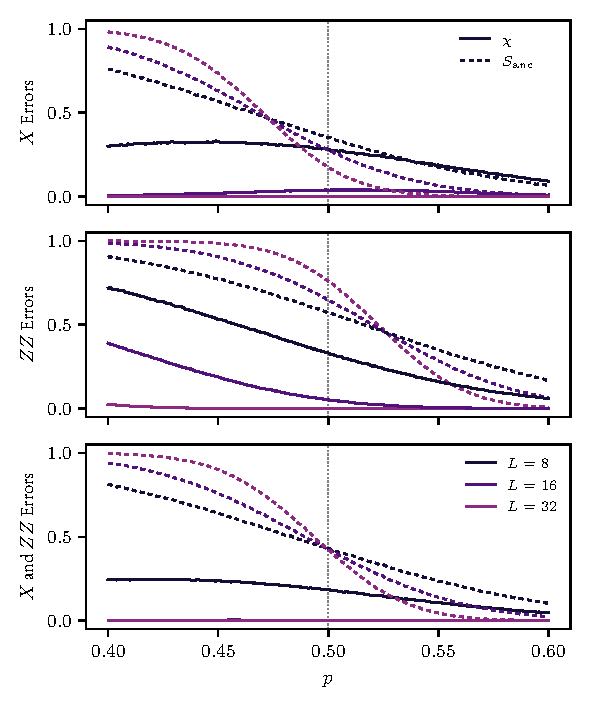
\includegraphics{anc_vs_lxe_new.pdf}
  \caption{Ancilla entanglement entropy and linear cross entropy for an error
  rate of $q=0.1$ to highlight the behavior of $S_\mathrm{anc}$. The system sizes are chosen smaller compared to
\cref{fig:err-vs-tra} since $\chi$ would be $0$ for larger systems. Note that
this is shown for the region around the critical point $p=0.5$ in the ideal
case. This was done to make the shift of $S_\mathrm{anc}$ in $p$ more
noticeable without having the cross entropy be $0$ for small
system sizes. Grey vertical dots indicate the critical point in the ideal case
of no errors at $p = 0.5$. Each datapoint corresponds to the sampling of $\sim 10^5$ circuit realizations.}
  \label{fig:large-q-anc-vs-lxe}
\end{figure}

\subsection{Marginalization}
\label{sec:lxe-err-subset} 
Notice that if, instead of applying projection operations, we applied
measurement gates in the right hand side circuits depicted in
\cref{fig:mech-b1-lxe,fig:mech-b2-lxe}, we would -- obviously -- not project
onto the 0-vector, and thus the circuit would continue. This is exactly what
happens when one marginalizes out the measurement results of $ZZ$ or $X$
measurements, as discussed in \cref{sec:lxe-indep}.  It thus stands to reason
that we should entertain this probability theoretic trick for the noisy
circuits.

Within $\tilde{C}$ and $C$ the same argument as in
\cref{sec:lxe-indep} holds. The outcomes we track are still independent
random variables, now only with a different circuit that produces them,
i.e. 
\begin{align}
  P(\mathbf{m}_X \cap \mathbf{m}_Z | \tilde{C}, \rho) = 
  P(\mathbf{m}_X | \tilde{C}, \rho)\cdot P(\mathbf{m}_Z | \tilde{C}, \rho)
.\end{align}

Therefore, despite the fact that $\rho$ and $\sigma$ are being subjected to physically
different circuits, we can still separate the respective probabilities as we
did before. We just need to be careful with the interpretation. That is, we can
follow the derivation in \cref{eq:lxe-subset}, where we replace $C$ in the
probabilities conditioned on initial state $\rho$ with $\tilde{C}$,

\begin{align}
      \label{eq:lxe-subset-err}
      \chi_{\tilde{C},C} &= \sum_{\mathbf{m}} P(\mathbf{m} \mid \tilde{C}, \rho) \frac{P(\mathbf{m} \mid
      C, \sigma)}{\sum_{\mathbf{m}'}\left(P(\mathbf{m}' \mid
      C, \sigma)\right)^2} \nonumber\\
      \nonumber\\
      &= \sum_{\mathbf{m}_X \cap \mathbf{m}_Z} P(\mathbf{m}_X \cap \mathbf{m}_Z |
        \tilde{C}, \rho) \frac{P(\mathbf{m}_X \cap \mathbf{m}_Z| C,
        \sigma)}{\sum_{\mathbf{m}_X' \cap \mathbf{m}_Z'} \left(P(\mathbf{m}_X' \cap
        \mathbf{m}_Z'|C,\sigma)\right)^2}\nonumber\\
        \nonumber\\
      &= \sum_{\mathbf{m}_X \cap \mathbf{m}_Z} P(\mathbf{m}_X | \tilde{C}, \rho) P(
        \mathbf{m}_Z | \tilde{C}, \rho) \frac{P(\mathbf{m}_X | C, \sigma) P( \mathbf{m}_Z|
        C, \sigma)}{\sum_{\mathbf{m}_X' \cap \mathbf{m}_Z'}
          \left(P(\mathbf{m}_X' | C,
        \sigma) P( \mathbf{m}_Z'|C,\sigma)\right)^2}\nonumber\\
        \nonumber\\
      &= \underbrace{\frac{\sum_{\mathbf{m}_Z} P(\mathbf{m}_Z | \tilde{C}, \rho)
          P(\mathbf{m}_Z | C, \sigma)}{\sum_{\mathbf{m}_Z'}
          \left(P(\mathbf{m}_Z' |
          C, \sigma)\right)^2}}_{\text{Subset ZZ}}
          \underbrace{\frac{\sum_{\mathbf{m}_X} P(\mathbf{m}_X | \tilde{C}, \rho)
          P(\mathbf{m}_X | C, \sigma)}{\sum_{\mathbf{m}_X'}
          \left(P(\mathbf{m}_X' |
          C, \sigma)\right)^2}.}_{\text{Subset X}}
\end{align}

As discussed previously, by tracing out the other measurement outcomes, we
effectively replace them by an identity in the calculation of the probability.
It therefore turns out that tracking only the outcomes $\mathcal{O}$-measurements prevents us from
seeing $\mathcal{O}$-errors. Another way one can convince oneself of this fact
is the following.
If we do not care about the outcomes of the observable, where no errors
happen, then every error gets necessarily bypassed as described above. We can
no longer distinguish if a measurement turned from random to deterministic due
to a faulty random measurement. The outcome is still a valid one with respect to
$C$ (and possibly $\sigma$, for that matter). On the other hand, it will be
impossible to tell if the initial entanglement cluster died because of a faulty
measurement or a native one. 

In particular will marginalizing over $ZZ$, i.e. tracking $X$, with $X$-errors
yield the identical linear cross entropy as in the noiseless case. With the
results of \cref{sec:lxe-indep} we also know that this is then equivalent to
tracking every outcome in the noiseless circuit.
Furthermore will tracking
$ZZ$ while having $ZZ$ errors still be identically $1$. 
Note that this implies that the different mechanisms for the different error
types get absorbed depending on which observable we choose to keep track of. 

\subsubsection{Results}
The results of the numerical analysis are shown in \cref{fig:err-vs-tra}. The
linear cross entropy and the entanglement entropy of an ancilla qubit are shown,
where every possible combination of error type and marginalization is represented in
a separate subplot. Although we previously made reference to the figure, we
will clarify how the tableau presentation is to be read, as we will employ it
again for our numerical results in \cref{ch:rel-ent}.

Along the rows of the
tableau of subplots we simulate the PTIM with noise represented by different
observables. In the first row, there are no errors, $q=0$. In the second row,
we introduce symmetric noise in $X$ as defined in
\cref{sec:errormodel,eq:noisechannel}. As error rate we choose $q=0.01$ in
agreement with Ref. \cite{tikhanovskayaUniversalityCrossEntropy2023}. In the
third row we proceed analogously with $ZZ$ errors, also at a rate of $q=0.01$.
In the last row, we combine the two, where first the noise channel of $X$ and
then the one of $ZZ$ is applied. 

Along the columns of \cref{fig:err-vs-tra}, we use a different subset of
measurement outcomes. In the first column, titled \enquote{Track X}, we track
the outcomes of $X$ measurements, and replace projections onto $ZZ$ results
with measurement operations. The second column, titled \enquote{Track ZZ} is
the converse of the first, with $ZZ$ outcomes tracked and $X$ outcomes
marginalized. The last column is where we track everything. 

The solid line denotes the linear cross entropy, while the dashed line is the
ancilla entanglement entropy. Note that each simulation was done twice: once
for an isolated system, which we then compared with $\sigma$ in order to
compute the linear cross entropy, and another one entangled to an ancilla
qubit.  We want to emphasize that the different combinations of errors and
marginalizations are qualitatively different in that some system sizes need not
be shown for one or the other. For instance, in the \enquote{X Errors, Track
all} case, the linear cross entropy for $L=64$ would be $0$ almost everywhere,
with miniscule deviations. We thus omit some system sizes in some subplots,
also in an effort to retain legibility.

Within each subplot we annotated each curve to qualitatively indicate the
predominant mechanism that sends $\chi$ to $0$, refering to the previously
defined denotions of said mechanism. For the \enquote{$X$ Errors -- Track $X$},
\enquote{No Errors -- Track $X$}, and \enquote{No Errors -- Track all}
situations, the only mechanism is the one where the initial cluster dies by
means of an $X$ measurement. As such, mechanism \textsf{A} is the predominant
one. For the \enquote{$X$ Errors -- Track all}, we have \textsf{A}, as well as
\textsf{B1}, the latter of which is predominant in the regime $p<p_c$, whereas
the former is predominant for $p> p_c$. Notice that this can be seen in the
combination of the subplots to the left of it. In the \enquote{No Errors --
Track $ZZ$} case, the linear cross entropy is identically $1$, which is no
longer the case for $X$ errors. Here, we have \textsf{B1}, which is the only
mechanism by which the $ZZ$ linear cross entropy goes to 0.

Since we also know that the \enquote{Track all} linear cross entropy is the
product of the marginalized ones, we can read each line as the product of the
first two plots equaling the third one. For rows 1 and 3, this is rather
trivial. For the others, it offers an explanation as to why it was necessary to
lower the system size in the last column.\footnote{The last row offers the
better visualization of this phenomenon in the nontrivial case compared to the
second.} This shows that the simulations agree with the prediction.

These remarkable results notwithstanding, we would still be hard-pressed to
find any evidence of the \emph{real}, i.e. \emph{measureable}, phase transition
of the projective transverse-field Ising model in noisy systems. This is highlighted by the fact
that the \enquote{true} behavior of the system is simulated as well in the form
of the ancilla entanglement entropy. For this we especially focus on the last
row of the tableau, which would be the noisiest system, where the behavior of
the linear cross entropy is seemingly decoupled from the dynamics of the
cluster. In particular, due to the exponential suppression in the
thermodynamic limit the mechanisms that are \emph{not} \textsf{A} dominate.  

However, this exponential suppression can be synthesized
%\footnote{in the Hegelian sense} 
into an advantage. Notice that as a consequence of this
suppression, the \enquote{Track $ZZ$} column is highly sensitive to $X$ noise.
Where it is identically $1$ in the ideal case, even small error rates in small
systems lead to the deviation from the ideal behavior. We can therefore use
this fact, as well as \cref{eq:lxe-estimate}, to estimate how noisy our system
is. As such, one \emph{could} still draw some utility from the linear cross
entropy, in that the \enquote{Track $ZZ$} column could function as an indicator
of noise in the system, albeit only noise in $X$, i.e. bitflips. 

%Inside the plots are annotations which qualitatively indicate the mechanism
%behind $\chi$ going to $0$, refering to the previously defined denotions of
%said mechanisms. 
%At the end of each circuit simulation, we computed the entanglement entropy of
%the ancilla. It is $1$ if the cluster survived and $0$ otherwise. Its critical
%point should be lower for $X$ errors, higher for $ZZ$ errors and roughly equal
%to the ideal case for $X$ and $ZZ$ errors.  \Cref{fig:large-q-anc-vs-lxe}
%offers a visualization of this phenomenon.  One can, of course, combine the
%lot ad absurdum, which culminates into \cref{fig:err-vs-tra}, with the quest
%of finding a worthy representative of the actual happenings inside the PTIM.
%
%\Cref{fig:err-vs-tra} shows multiple plots of $\chi$ as a function of $p$,
%where $p$ ($1-p$) is the probability of a single-site $X$ ($ZZ$) measurement.
%The plots are ordered as follows. In each row there is some kind of error
%present: none, $X$, $ZZ$, and $X$ and $ZZ$. Each error happens at an error
%rate of $q=0.01$. In each column, we track a different subset of measurements,
%$X$, $ZZ$, and all measurements.

%\Cref{fig:err-vs-tra} hopefully looks nice. Maybe it also floats to the correct
%place!
\begin{figure}[p]
  \centering
  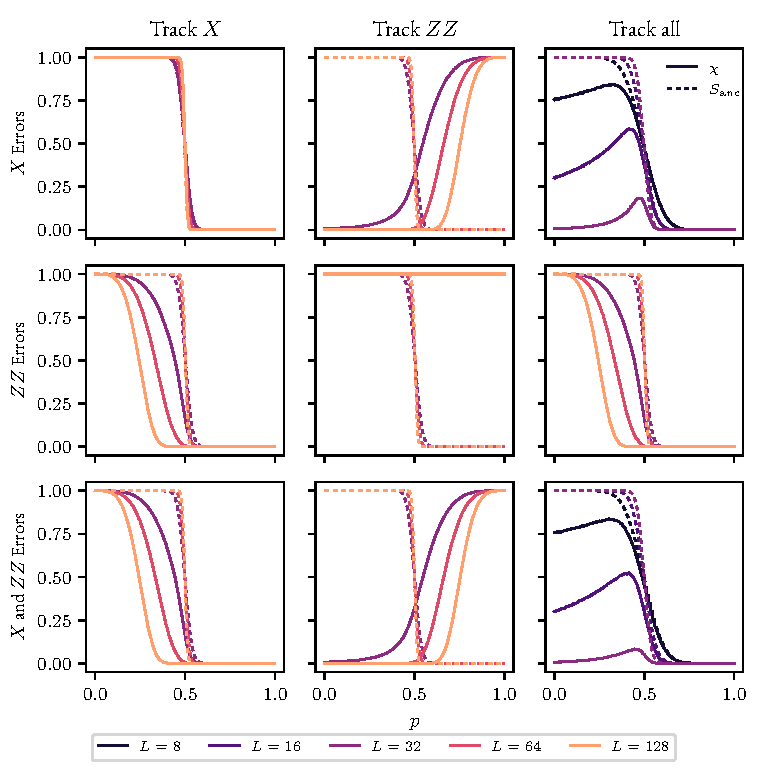
\includegraphics{errors-vs-tracked.pdf}
  \caption{Linear cross entropy (solid) and entanglement entropy of an ancilla qubit
  entangled to the initial cluster (dashed) for $p\in[0,1]$ for all combinations of
errors and marginalizations and different system sizes. Note that the ancilla entropy is unaffected by the
marginalizations. Annotations within the subfigures reference the predominant mechanisms of
the linear cross entropy going to $0$. \textsf{A} corresponds to
\cref{fig:mechanism-a}, \textsf{B1} and \textsf{B2} correspond to
\cref{fig:mech-b1-lxe,fig:mech-b2-lxe}, respectively.}
  \label{fig:err-vs-tra}
\end{figure}
%It didn't seem to do so, so i passed \texttt{[h!]}
\newpage
\section{Summary}
In this chapter we examined the linear cross entropy in the projective
transverse-field Ising model. The linear cross entropy was introduced by
\citeauthor{liCrossEntropyBenchmark2023} in \cite{liCrossEntropyBenchmark2023},
and first investigated for the projective transverse-field Ising model by
\citeauthor{tikhanovskayaUniversalityCrossEntropy2023} in
\cite{tikhanovskayaUniversalityCrossEntropy2023}. In search of a promising
candidate for an order parameter of the phase transition that is measureable in
an experimental setting, we picked up where these previous works left off. Our investigations
showed that while it is a fitting quantity for noiseless systems, the linear
cross entropy is not at all robust to noise in the system, as it gets exponentially
suppressed with larger system size. We additionally showed that we can
marginalize over measurement outcomes of one operator and still find some
utility in the linear cross entropy. In an experimental setting, the
marginalized linear cross entropy could be employed in attempts to minimize the
influence of noise, as it is highly sensitive to noise.
